%%%%%%%%%%%%%%%%%%%%%%%%%%%%%%%%%%%%%%%%%%%%%%%%%%%%%%%%%%%%%%%%%%%%%%%%%%%%%%%%
% Template for USENIX papers.
%
% History:
%
% - TEMPLATE for Usenix papers, specifically to meet requirements of
%   USENIX '05. originally a template for producing IEEE-format
%   articles using LaTeX. written by Matthew Ward, CS Department,
%   Worcester Polytechnic Institute. adapted by David Beazley for his
%   excellent SWIG paper in Proceedings, Tcl 96. turned into a
%   smartass generic template by De Clarke, with thanks to both the
%   above pioneers. Use at your own risk. Complaints to /dev/null.
%   Make it two column with no page numbering, default is 10 point.
%
% - Munged by Fred Douglis <douglis@research.att.com> 10/97 to
%   separate the .sty file from the LaTeX source template, so that
%   people can more easily include the .sty file into an existing
%   document. Also changed to more closely follow the style guidelines
%   as represented by the Word sample file.
%
% - Note that since 2010, USENIX does not require endnotes. If you
%   want foot of page notes, don't include the endnotes package in the
%   usepackage command, below.
% - This version uses the latex2e styles, not the very ancient 2.09
%   stuff.
%
% - Updated July 2018: Text block size changed from 6.5" to 7"
%
% - Updated Dec 2018 for ATC'19:
%
%   * Revised text to pass HotCRP's auto-formatting check, with
%     hotcrp.settings.submission_form.body_font_size=10pt, and
%     hotcrp.settings.submission_form.line_height=12pt
%
%   * Switched from \endnote-s to \footnote-s to match Usenix's policy.
%
%   * \section* => \begin{abstract} ... \end{abstract}
%
%   * Make template self-contained in terms of bibtex entires, to allow
%     this file to be compiled. (And changing refs style to 'plain'.)
%
%   * Make template self-contained in terms of figures, to
%     allow this file to be compiled. 
%
%   * Added packages for hyperref, embedding fonts, and improving
%     appearance.
%   
%   * Removed outdated text.
%
%%%%%%%%%%%%%%%%%%%%%%%%%%%%%%%%%%%%%%%%%%%%%%%%%%%%%%%%%%%%%%%%%%%%%%%%%%%%%%%%

\documentclass[letterpaper,twocolumn,10pt]{article}
\usepackage{unix}

% to be able to draw some self-contained figs
\usepackage{tikz}
\usepackage{amsmath}

% inlined bib file
\usepackage{filecontents}

\usepackage{enumitem}

%-------------------------------------------------------------------------------
\begin{filecontents}{\jobname.bib}
%-------------------------------------------------------------------------------
@Book{arpachiDusseau18:osbook,
  author =       {Arpaci-Dusseau, Remzi H. and Arpaci-Dusseau Andrea C.},
  title =        {Operating Systems: Three Easy Pieces},
  publisher =    {Arpaci-Dusseau Books, LLC},
  year =         2015,
  edition =      {1.00},
  note =         {\url{http://pages.cs.wisc.edu/~remzi/OSTEP/}}
}
@InProceedings{waldspurger02,
  author =       {Waldspurger, Carl A.},
  title =        {Memory resource management in {VMware ESX} server},
  booktitle =    {USENIX Symposium on Operating System Design and
                  Implementation (OSDI)},
  year =         2002,
  pages =        {181--194},
  note =         {\url{https://www.usenix.org/legacy/event/osdi02/tech/waldspurger/waldspurger.pdf}}}
\end{filecontents}

%-------------------------------------------------------------------------------
\begin{document}
%-------------------------------------------------------------------------------

%don't want date printed
\date{}

% make title bold and 14 pt font (Latex default is non-bold, 16 pt)
\title{\Large \bf Formatting Submissions for a USENIX Conference:\\
  An (Incomplete) Example}

%for single author (just remove % characters)
\author{
{\rm Sabrina\ Brogren}\\
University of Michigan
\and
{\rm Christina Foshiem-Hoag}\\
University of Michigan
\and
{\rm Oliver Miles}\\
University of Michigan
} % end author

\maketitle

%-------------------------------------------------------------------------------
\begin{abstract} % 2-3 paragraphs
%-------------------------------------------------------------------------------
Multithreaded programs suffer from nondeterministic behavior ranging from data races to uninitialized variables. GPU (graphic processing unit) programs are especially vulnerable to bugs related to nondeterministic behavior due to their high level of paralellization. 
These bugs can be especially difficult to catch, as merely running the program again with the same inputs does not guarantee that the bug will rear its head again. 
Frameworks like PinPlay and Instant Replay allow a user to record and deterministically replay a program, but no tool yet exists with the same functionality for GPU programs. 


Our goal is to create a tool that allows a user to capture the execution of their GPU program and replay the execution. 
The source of nondeterminism we're focusing on is data races. 
We want to be able to replay a GPU program such that not only do threads interacting with memory run in the same order, but also the state of memory throughout the program is identical to when it was recorded. 
We used NVBit (NVidia Binary Instrumentation Tool) to instrument instructions that operate on memory (loads and stores). 
On record, we record all loads and stores. 
On replay, we use locks to replay the loads and stores for each memory address in order. 
This paper will describe the describes the design of our tool, as well as discusses its usage on racey GPU programs.
We hope our tool will serve as a proof of concept for further endeavors into GPU record and replay tools.
\end{abstract}


%-------------------------------------------------------------------------------
\section{Introduction - 1 page}
%-------------------------------------------------------------------------------

"Define and motivate the problem with examples, briefly talk about challenges. 
Explain your core high-level idea. 
Give an overview of your solution and summarize key results"
Discuss other solutions (none exist). Talk about other kinds of nondeterminism like multiple kernals, uninitialized memory. Describe the core concept, which is to get all values when recording and replay them in order.

Nondeterminism is the root of many complex bugs. The move to increasingly parallel programs

When a GPU program starts running on the CPU, the CPU uses the GPU for parallel computing by launching kernels onto it. Each of these kernels consists of threads, which are organized into uniformly-sized blocks. All threds in the kernel run the exact same kernel function, though their control flows may differ. Threads can access different kinds of memory. Every thread has its own register and local memory, which are only able to be accessed by that thread and only live for the lifetime of the thread. Shared memory is shared among threads in a block, which allow threads to communicate with each other. Finally, global memory is shared among all the threads in the application.

We decided to focus on data races specifically related to shared and global memory. Let's motivate this with an example program:

\begin{verbatim}
#include <stdio.h>

__global__ void saxpy(int n, float a, float *x, float *y) {
  int i = blockIdx.x*blockDim.x + threadIdx.x;
  if (i < n) y[i] = a*x[i] + y[i];
}

int main(void) {
  int N = 1<<20;
  float *x, *y, *d_x, *d_y;
  x = (float*)malloc(N*sizeof(float));
  y = (float*)malloc(N*sizeof(float));

  cudaMalloc(&d_x, N*sizeof(float)); 
  cudaMalloc(&d_y, N*sizeof(float));

  for (int i = 0; i < N; i++) {
    x[i] = 1.0f;
    y[i] = 2.0f;
  }

  cudaMemcpy(d_x, x, N*sizeof(float), cudaMemcpyHostToDevice);
  cudaMemcpy(d_y, y, N*sizeof(float), cudaMemcpyHostToDevice);

  // Perform SAXPY on 1M elements
  saxpy<<<(N+255)/256, 256>>>(N, 2.0f, d_x, d_y);

  cudaMemcpy(y, d_y, N*sizeof(float), cudaMemcpyDeviceToHost);

  float maxError = 0.0f;
  for (int i = 0; i < N; i++)
    maxError = max(maxError, abs(y[i]-4.0f));
  printf("Max error: %f\n", maxError);

  cudaFree(d_x);
  cudaFree(d_y);
  free(x);
  free(y);
}
\end{verbatim}

%-------------------------------------------------------------------------------
\section{Design - 3 pages}
%-------------------------------------------------------------------------------
GPlayU is composed of three stages: record, processing, and replay. 

\subsection{Record}


\subsection{Processing}
The result of the record stage was a file for each kernel. In the record stage, every interaction with memory was recorded (load or store) alongside its associated values (address, thread number, counter, and value that was loaded or stored). This data needs to be processed before feeding it to the replay stage. This is accomplished by a simple program written in C++14. Let's look at a short example output file from the record stage:

\begin{verbatim}
5 0x0c 1 S G 0xff
3 0x0c 2 S G 0x01
8 0x0c 5 L G 0x00
9 0x0c 5 L G 0xff

\end{verbatim}

Each line is has values in the order \texttt{count}, \texttt{address}, \texttt{thread\_id}, \texttt{store/load}, \texttt{global/shared}, and \texttt{value}. As this data is not going to be in order, the processing stage could simply order by \texttt{count} and print the data back out. The the replay stage would force load and store instructions to run in the exact same order on replay. However, this would incur a lot of unnecessary overhead.

In the example, thread 1 is loading from address \texttt{0x04} at count 1, then thread 2 is storing to address \texttt{0x0c} at count 3. Since these two threads operate on different locations in memory, enforcing the ordering of the two is not necessary. Potential data races can be examined and controlled in a more fine-grained manner by looking first at addresses, then the accesses to those addresses. The processing stage does not actually detect data races, but identifies addresses that may have write/write or write/read dependencies, and outputs the order of memory accesses to those addresses.

Therefore data must be organized first by address, and then by counter. The result of the processing stage is again a file for each kernal, organized by address. This stage must also account for the double loads output by the recording stage: when encountering the data for two loads by the same thread at the same address, the first datum contains the correct count, while the second contains the correct value.

The first line of processing output is how many addresses there are with potential data races. Then each line is composed of the addresses, the number of memory operations on that address, followed by a tuple of \texttt{thread\_id}, \texttt{store/load}, and \texttt{value}. Here is the output from the sample:

\begin{verbatim}
1
0x0c 3 2 S 0x01 1 S 0xff 5 L 0xff
\end{verbatim}

There are also a couple simple optimizations in this stage that make a big difference in output file size, especially when run on larger programs. To reiterate, GPlayU is designed to preserve the state of memory after the replay of a program by controlling for data races, so all optimizations were made within these constraints. Here is some sample record output to show the optimizations:

\begin{verbatim}
1 0x10 1 L G 0x00
2 0x10 1 L G 0x00
3 0x10 2 L G 0x00
4 0x10 2 L G 0x00
5 0x0c 1 S G 0xff
6 0x0c 1 S G 0x00
7 0x04 2 S G 0xff
8 0x04 3 S G 0xff
9 0x1c 3 S G 0xff
\end{verbatim}
There are four different optimizations at each of the memory addresses in the sample output that altogether result in the processing stage reporting no potential data races.

\begin{description}[font=$\bullet$\scshape\bfseries]
\item [Only Loads] The only memory operations on the address \texttt{0x10} are loads. Since there are no stores actually changing the value at this memory address, it is unnecessary to output these loads.
\item [Same Thread] At address \texttt{0x0c}, there are two stores executed by the same thread. Within threads, instructions are executed sequentially, so these two stores will always be in the same order. Therefore, if all the memory operations at a certain address are executed by the same thread, there are no data races.
\item [Same Value] At address \texttt{0x04}, there are two stores executed by different threads. However, the threads are storing the same values, so it doesn't matter which thread executes the store first. 
\item [One Operation] At address \texttt{0x1c}, there is only one memory operation. There is only one possible ordering with one operation, so this is not a data race.
\end{description}

\subsection{Replay}
Similar to the record stage, the replay stage also necessitates instrumenting all loads and stores. Additionally, the replay stage needs to take the output of processing, read it in on the host, and distribute it to the device, where thread ordering will be enforced. Data is read into a two-dimensional array on the host and then copied to the device for use in replaying.

At each load or store, the relevant memory address is checked to see if there are any dependencies associated with it. If so, the thread checks if it is the next to be run. This information is stored in device array, and the lock is not needed to read it. When the thread is next to be run, it grabs the lock, which is global to all threads. While in posession of the lock, the thread does the following: it first executes the load or store with the value saved in the device array by manually moving the value into memory or a register. Then it updates the value of the next thread to be run.

The instrumentation functions for load and store instructions are called before the instruction executes. The execution order of these instructions must be controlled, so they replay stage cannot simple let go of the lock after asserting that it is that thread's turn to execute and leave the thread to run the subsequent load or store. The actual instruction must be deleted and manually executed while holding the lock.

Using NVBit and Cuda.
What was instrumented and recorded?
What challenges did we face? (ASLR, had to use a count to keep track of order when recording, had to implement our own locks, needed to manually replay loads and stores to make sure order is maintained)
What other design decisions have we considered (replaying just by inserting data values, but not maintaining ordering. This gives us the same output from a program, but does not replay memory as well.)

%-------------------------------------------------------------------------------
\section{Implementation - 0.5 page}
%-------------------------------------------------------------------------------

"Explain subtle implementation details"
-Explain how we implemented a lock?

%-------------------------------------------------------------------------------
\section{Evaluation}
%-------------------------------------------------------------------------------

"Convince the reader that your system works and explain when it fails"
8-9 benchmarks
discuss overhead (maybe look at overhead with only loads/only stores)

%-------------------------------------------------------------------------------
\section{Related Work - 0.5-1 page}
%-------------------------------------------------------------------------------

Pin-Play
How is our work the same? How is it the same? What ideas were adopted from other works?

Our work, however, is certainly not the first to be done on GPUs and determinism. In 2013, GPUDet was released as the first massively parallel and strongly deterministic architecture. It guarantees determinism by only allowing threads to communicate at fixed, deterministic intervals. 

%-------------------------------------------------------------------------------
\section{Discussion - 0.5 page}
%-------------------------------------------------------------------------------

"Discuss your limitations and possible workarounds"

%-------------------------------------------------------------------------------
\section{Conclusion - 2-3 paragraphs}
%-------------------------------------------------------------------------------

"Summarize your paper and breifly point out the future work"

Future work - actually doing something different with shared vs global.

%-------------------------------------------------------------------------------
\section{Footnotes, Verbatim, and Citations}
%-------------------------------------------------------------------------------

Footnotes should be places after punctuation characters, without any
spaces between said characters and footnotes, like so.%
\footnote{Remember that USENIX format stopped using endnotes and is
  now using regular footnotes.} And some embedded literal code may
look as follows.

\begin{verbatim}
int main(int argc, char *argv[]) 
{
    return 0;
}
\end{verbatim}

Now we're going to cite somebody. Watch for the cite tag. Here it
comes. Arpachi-Dusseau and Arpachi-Dusseau co-authored an excellent OS
book, which is also really funny~\cite{arpachiDusseau18:osbook}, and
Waldspurger got into the SIGOPS hall-of-fame due to his seminal paper
about resource management in the ESX hypervisor~\cite{waldspurger02}.

The tilde character (\~{}) in the tex source means a non-breaking
space. This way, your reference will always be attached to the word
that preceded it, instead of going to the next line.

And the 'cite' package sorts your citations by their numerical order
of the corresponding references at the end of the paper, ridding you
from the need to notice that, e.g, ``Waldspurger'' appears after
``Arpachi-Dusseau'' when sorting references
alphabetically~\cite{waldspurger02,arpachiDusseau18:osbook}. 

It'd be nice and thoughtful of you to include a suitable link in each
and every bibtex entry that you use in your submission, to allow
reviewers (and other readers) to easily get to the cited work, as is
done in all entries found in the References section of this document.

Now we're going take a look at Section~\ref{sec:figs}, but not before
observing that refs to sections and citations and such are colored and
clickable in the PDF because of the packages we've included.

%-------------------------------------------------------------------------------
\section{Floating Figures and Lists}
\label{sec:figs}
%-------------------------------------------------------------------------------


%---------------------------
\begin{figure}
\begin{center}
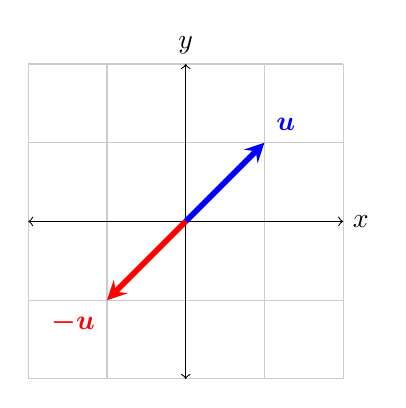
\begin{tikzpicture}
  \draw[thin,gray!40] (-2,-2) grid (2,2);
  \draw[<->] (-2,0)--(2,0) node[right]{$x$};
  \draw[<->] (0,-2)--(0,2) node[above]{$y$};
  \draw[line width=2pt,blue,-stealth](0,0)--(1,1)
        node[anchor=south west]{$\boldsymbol{u}$};
  \draw[line width=2pt,red,-stealth](0,0)--(-1,-1)
        node[anchor=north east]{$\boldsymbol{-u}$};
\end{tikzpicture}
\end{center}
\caption{\label{fig:vectors} Text size inside figure should be as big as
  caption's text. Text size inside figure should be as big as
  caption's text. Text size inside figure should be as big as
  caption's text. Text size inside figure should be as big as
  caption's text. Text size inside figure should be as big as
  caption's text. }
\end{figure}
%% %---------------------------


Here's a typical reference to a floating figure:
Figure~\ref{fig:vectors}. Floats should usually be placed where latex
wants then. Figure\ref{fig:vectors} is centered, and has a caption
that instructs you to make sure that the size of the text within the
figures that you use is as big as (or bigger than) the size of the
text in the caption of the figures. Please do. Really.

In our case, we've explicitly drawn the figure inlined in latex, to
allow this tex file to cleanly compile. But usually, your figures will
reside in some file.pdf, and you'd include them in your document
with, say, \textbackslash{}includegraphics.

Lists are sometimes quite handy. If you want to itemize things, feel
free:

\begin{description}
  
\item[fread] a function that reads from a \texttt{stream} into the
  array \texttt{ptr} at most \texttt{nobj} objects of size
  \texttt{size}, returning returns the number of objects read.

\item[Fred] a person's name, e.g., there once was a dude named Fred
  who separated usenix.sty from this file to allow for easy
  inclusion.
\end{description}

\noindent
The noindent at the start of this paragraph in its tex version makes
it clear that it's a continuation of the preceding paragraph, as
opposed to a new paragraph in its own right.


\subsection{LaTeX-ing Your TeX File}
%-----------------------------------

People often use \texttt{pdflatex} these days for creating pdf-s from
tex files via the shell. And \texttt{bibtex}, of course. Works for us.

%-------------------------------------------------------------------------------
\section*{Acknowledgments}
%-------------------------------------------------------------------------------

The USENIX latex style is old and very tired, which is why
there's no \textbackslash{}acks command for you to use when
acknowledging. Sorry.

%-------------------------------------------------------------------------------
\section*{Availability}
%-------------------------------------------------------------------------------

USENIX program committees give extra points to submissions that are
backed by artifacts that are publicly available. If you made your code
or data available, it's worth mentioning this fact in a dedicated
section.

%-------------------------------------------------------------------------------
\bibliographystyle{plain}
\bibliography{\jobname}

%%%%%%%%%%%%%%%%%%%%%%%%%%%%%%%%%%%%%%%%%%%%%%%%%%%%%%%%%%%%%%%%%%%%%%%%%%%%%%%%
\end{document}
%%%%%%%%%%%%%%%%%%%%%%%%%%%%%%%%%%%%%%%%%%%%%%%%%%%%%%%%%%%%%%%%%%%%%%%%%%%%%%%%

%%  LocalWords:  endnotes includegraphics fread ptr nobj noindent
%%  LocalWords:  pdflatex acks
